
\section{Live Processing}

\subsection{Introduction}

The SNS collects event mode data on all of it's instruments, and ISIS is also beginning to roll out event mode data capture.  One of the benefits of event mode data is the ability to make changes to an experiment quickly based on the results collected so far.  Scientist would benefit greatly from being able to visualise reduced data in 'real' time, or close to 'real' time.  This may also be extended later to allow integration with the instrument control to allow automated decisions to be made on the analysis of live data.

In this section we will describe the detailed design of the components required for live event data analysis of the Mantid Framework.  It is based on the design of the Mantid Framework specified in the Architectural Design Document [ADD].
It will form the basis of the development of this aspect of the framework and act as a guide for maintaining the system.

\subsection{Overview}

\begin{figure}[h!]
\centering
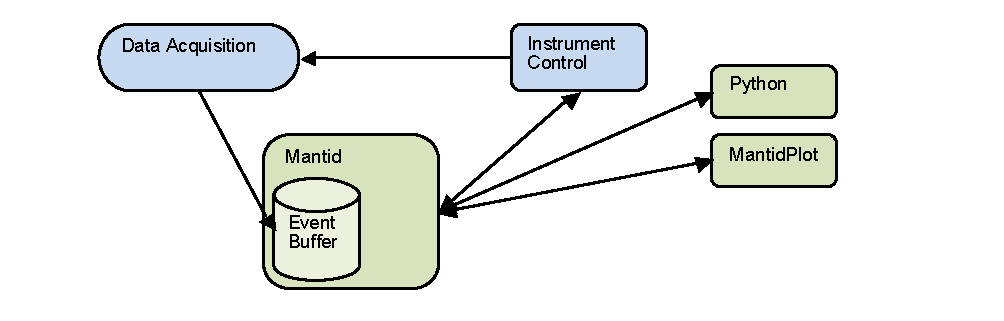
\includegraphics{overview_diagram}
\end{figure}

The Diagram above show an overview of the proposed design encompassing all of the systems involved.  The data acquisition sends all event information in response to requests from Mantid or other applications.  Mantid stores data to be processed in an internal event buffer  until it is ready to process a 'batch' of events.  Mantid is responsible for the processing of the data received and amalgamating it with any data already processed.  This can then be used either in Python or visualised using Mantidplot.  In the future we could "close the loop" by allowing instrument control scripts to drive this process and respond to the results from the processed data, for example, The sample could be rotated to the next position once the processed data passes a set signal to noise ratio.

\subsection{Mantid Processing of Live Data}

In order to efficiently process live event data it would be important to only process the events that have been added since the last call to the event buffer, this can then be accumulated in a result dataset for display or further analysis. The diagram below shows a potential design that would allow this processing of 'live' data.

\begin{figure}[h!]
\centering
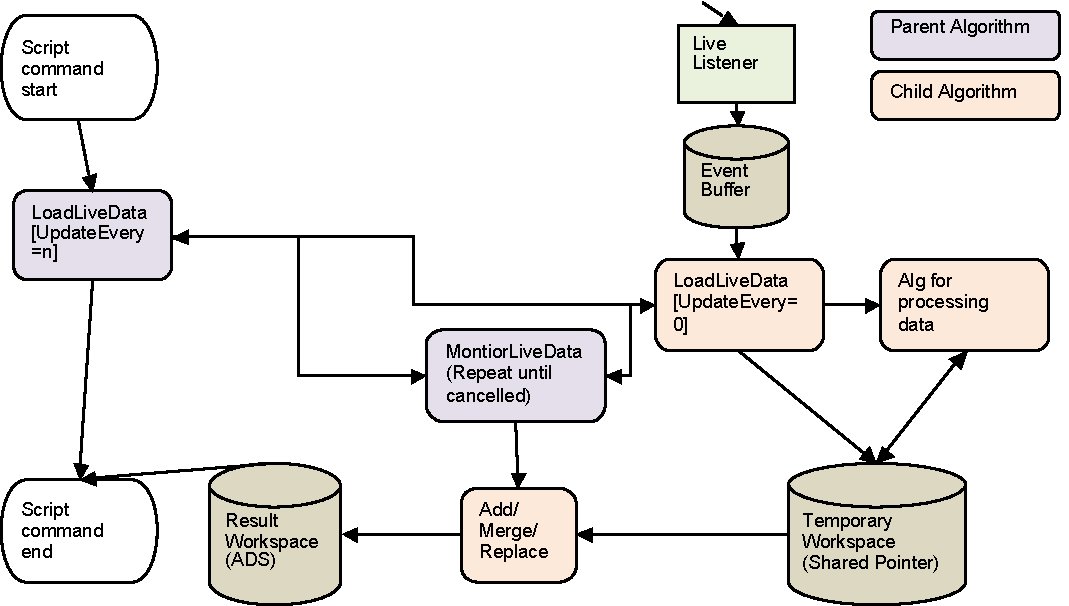
\includegraphics{processing_diagram}
\end{figure}

\subsubsection{Process Flow}
\begin{enumerate}
\item LoadLiveData With UpdateEvery property set to a value starts, spawns a child algorithm of LoadLiveData with UpdateEvery =0
\item LoadLiveData [UpdateEvery=0] Loads the info from the event feed into a workspace
\item LoadLiveData [UpdateEvery =0] creates and executes as a child algorithm the specified algorithm for processing
\item The resulting workspace is fed back to LoadLiveData [repeat=true] and set as the output workspace
\item LoadLiveData [UpdateEvery =n] create MonitorLiveData as a Parent Algorithm
\item LoadLiveData [UpdateEvery =n] ends.
\item MonitorLiveData  spawns a child algorithm of LoadLiveData with UpdateEvery =0 loading into a temporary (shared pointer) workspace
\item Steps 2 and 3 are repeated
\item The resulting workspace is fed back to MonitorLiveData
\item MonitorLiveData uses the Add child algorithm to add or merges the contents of the temporary workspace 
to the result workspace
\item Update signals from the altered result workspace will replot any graphs.
\item Unless cancelled MonitorLiveData starts again from step 7.
\end{enumerate}

\subsubsection{Benefits}

\begin{enumerate}
\item Control is returned to any script as soon as the first "chunk" of data has completed processing, allowing any graphs to be created in python.
\item The looping is controlled in only one algorithm, which can be cancelled by normal means.
\item Loading and the spawning of any processing is encapsulated in one algorithm.
\item Using Child algorithms and shared pointer workspaces will allow for memory to be cleared up as soon as it is no longer needed.
\end{enumerate}


\subsection{Algorithms}

\subsubsection{LoadLiveData}
The LoadLiveData algorithm provides a user interaction point to setup live data monitoring.  It also understands how to load the data from an event buffer and can manage the processing of the data through whatever user defined algorithm is requested.

In order for the user interaction to be flexible enough to cope with whatever user defined processing algorithm is used the properties of this algorithm need to be very flexible, as different processing algorithms may require different input properties to be set.  Fortunately we already have a model for this within Mantid, The Load Algorithm has a few set properties, and then inherits the additional properties that are specific to the data loader selected.  Thus similarly LoadLiveData will have certain fixed properties:

\begin{enumerate}
\item Instrument: e.g. GEM, CNCS
\item OutputWorkspace
\item StartSpectrumNo
\item EndSpectrumNo
\item SpectrumList
\item LoadEventsFrom – a timestamp
\item UpdateEvery n seconds - 0 or blank means no updates.
\item ProcessingAlgorithm - A List of all applicable algorithms, can be left blank.
\item AccumulationAlgorithm - Short List of Add/Merge/Conjoin/Replace, default Add.  This will have no effect if UpdateEvery is set to 0.
\end{enumerate}

The Start, End and SpectrumList properties may not be implemented as they will not improve the loading speed for Event data, although they would improve the subsequent processing time.
In addition to these properties any additional properties from the selected ProcessingAlgorithm algorithm would be added at runtime to the LoadLiveData algorithm, with the exception of the following:
\begin{enumerate}
\item InputWorkspace - This will be programmatically set to be the shared pointer of the freshly loaded event workspace.
\item OutputWorkspace - This will be programmatically extracted from the completed algorithm as a shared pointer and fed into the AccumulationAlgorithm.
\end{enumerate}

In addition to OutputWorkspace it will also output the following property:
\begin{enumerate}
\item LastEventTimestamp - The timestamp of the last event (or possibly frame) loaded
\end{enumerate}


\subsubsection{MonitorLiveData}

The MonitorLiveData algorithm is responsible for managing the repeated execution of LoadLiveData and the accumulation of the results.  The properties of MonitorLiveData will mirror those of LoadLiveData, including any dynamically added properties.  MonitorLiveData will not itself use many of the properties, just pass them on to child algorithms.  MonitorLiveData will follow a simple set of steps repeatedly until it is cancelled:

\begin{enumerate}
\item Sleep for the number of seconds in UpdateEvery
\item Check if the algorithm has been cancelled
\item Launch a LoadLiveData algorithm with UpdateEvery=0, and LoadEventsFrom set to LastEventTimestamp from the last execution of LoadLiveData and extract the pointer to the outputworkspace.
\item Check if the algorithm has been cancelled
\item Launch the ProcessingAlgorithm (if one was set), and extracting the resulting output workspaces as pointers.
\item Check if the algorithm has been cancelled
\item Store the interim workspaces as hidden workspaces in the ADS, create a group workspace as necessary.
\item Launch the selected AccumulationAlgorithm adding the interim workspaces to the OutputWorkspace.
\item Remove any interim workspaces and group workspaces from the ADS.
\item Check if the algorithm has been cancelled
\item Loop back to step 1.
\end{enumerate}


Steps 9 and 11 are currently necessary because GroupWorkspaces do not hold a shared pointer to their child workspaces.  As such they cannot be returned effectively from child algorithms.  If we were to change this steps 9 and 11 may no longer be necessary.



\subsubsection{ProcessingAlgorithm}
The ProcessingAlgorithm can be any algorithm in Mantid that accepts and returns a workspace.  In most cases it will itself be a workflow algorithm that organises the work of several other "child" algorithms.  In many cases Python algorithms will be particularly suited to this task.  In all cases the first discovered InputWorkspace algorithm will be set to the interim event workspace that has been read from the data buffer, and all OutputWorkspace properties will be extracted as workspaces of interest.
It is perfectly possible to output more than one output workspace from the processing Algorithm, and indeed you can add more output workspaces at run time.  You should not however to change the number or order of workspaces returned during repeated "reads" of the same run.


\subsubsection{AccumulationAlgorithm}
The AccumulationAlgorithm is one of a short list of algorithms that perform the accumulation of the interim results workspace with the final results workspace.  Most of these algorithms are binary algorithms, with the exception of RenameWorkspace which will overwrite the existing data each time with the most recent 'batch' of live data.  All of the possible AccumulationAlgorithms need to be checked that they will operate correctly with GroupWorkspaces.

\subsection{Live Listeners}
The live data Listener classes will be responsible for setting up communication with the relevant data acquisition and translating the response into a common format for storage in the event buffer.  Differences between the data acquisition at different institutions will require different implementation of Live data listeners, but these will conform to the same ILiveListener interface and be delivered from a dynamic factory in a similar way to algorithms and units.  This will allow additional LiveListeners to be added as plugins to support other facilities or local changes.  The Facilities.xml file will be extended to include details of which LiveListener to use for each instrument and the socket connection details.

\begin{figure}[h!]
\centering
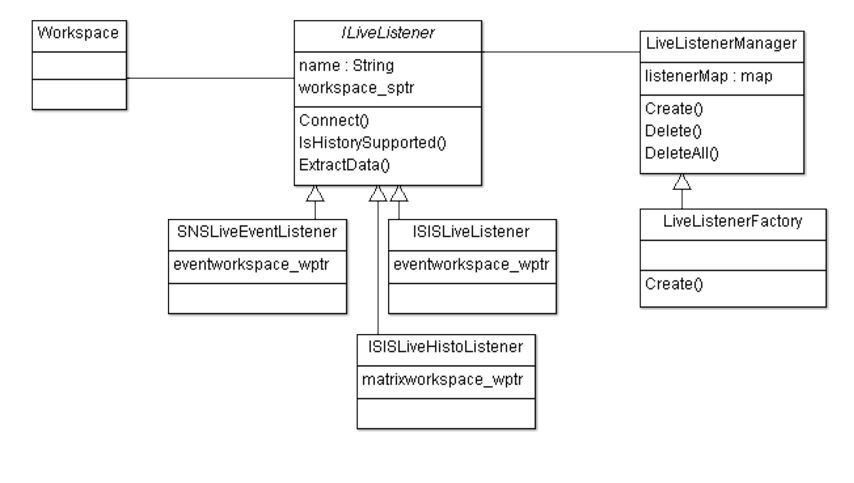
\includegraphics{LiveListeners}
\end{figure}

The ExtractData method will create an empty copy of the Workspace for use as a new event buffer, and then prepare the full event buffer for analysis.  This preparation may include adding log values, sorting event lists etc.

\subsubsection{Live Listener Factory} 
The listener factory is responsible for the creation of listeners by name, all listeners are returned as shared pointers.  This works in a similar way to the AlgorithmFactory.

\subsubsection{Live Listener Manager}
The Live Listener Manager inherits from the LiveListenerFactory and adds Lifetime management to the LiveListeners created.  This will work in a similar way to the Algorithm Manager for algorithms.  The Manager class maintains a map of all of the listeners created, so if another request is made for the same listener and connection details then the already existing object will be returned rather than creating a new listener.  For any new listeners that are created by the factory the connection to data acquisition will be established before the Listener is returned or stored internally.

\subsubsection{Live Listener Lifetime}
The LiveListener class will be kept alive by the ListenerManager class so it can be used across different instances of algorithms without going completely out of scope.  The following classes are responsible for managing the lifespan of the class in the Manager.
\begin{itemize}
\item LoadLiveData (whatever updateevery is set to) will call create on the Manager class.
\item LoadLiveData (updateevery = 0 and a parent algorithm) will call delete on the Manager class as the end of exec. This is the case where the user asked for a single run of the algorithm.
\item MonitorLiveData will call delete on the Manager class when it has been cancelled. This is the case where the user asked for an updating live feed.
\item ClearAllMemory will call DeleteAll on the Manager, removing all LiveListeners
\end{itemize}

Each Live Listener is responsible for releasing all memory (including workspaces) and sockets during it's destructor.



\subsection{Event Buffer}
The event buffer is a collection of data that is waiting to be processed. It is used as a temporary store by the Live Listener.  The Live Listener class will be responsible for monitoring the size of the buffer, and dropping data if necessary.  In reality it may make a lot of sense for this data store to be a Workspace itself, in which case no conversion would be required when the data is requested for processing.  For LiveListeners of event data it makes sense to se an EventWorkspace, initially with the event lists unsorted, and then only sort them when the data is being extracted from the Listener.  For LiveListeners of Histogram data it would make sense to use a MatrixWorkspace and only request the data from DataAcquisition when the data is being extracted.

\subsection{Data Acquisition Implementations}

\subsubsection{SNS}
At the SNS, the Data Acquisition system will provide the ability to serve events from a choice of three starting points.
\begin{enumerate}
\item The last run status change event (usually the run start, but it could be the run end.
\item The last 'checkpoint' during the run.  This will be on the order of every few minutes, so for a given time request the system will start from the first older check point than the time requested.  It will be up to Mantid to filter out the events from this checkpoint up to the time requested.
\item Start from the live stream.  This will not include any 'historical' events. 
\end{enumerate}

\subsubsection{ISIS}
The current plan for the ISIS implementation of a live event feed from the data acquisition feed is simpler, but more limited.  The data acquisition machine will accept a TCP socket from programs to "listen" to the live stream of events.  This will not include any ability to access the history of a run.  Similar functionality to that of the SNS may be added at a later date.

\subsection{Prioritization of Common Reduction Operators}

The order in which we will address the standard reduction for data streaming is as follows:

\begin{enumerate}
\item $I(Q)$ or $I(d)$ for non-crystalline diffraction.
\item $I(Q)$ for small angle scattering.
\item $I(Q,\omega)$ for inelastic scattering.
\end{enumerate}